\documentclass[a4paper, oneside, 11pt]{scrartcl}

% Get the necessary Packages
% Set to english language and utf8.
\usepackage[english]{babel}
\usepackage[utf8]{inputenc}

% Some packages for symbols we need within the tutorial.
\usepackage{dingbat}
\usepackage{marvosym}

% For the sourcecode.
\usepackage{listings}

% For the links etc.
\usepackage[pdfborder={0 0 0}]{hyperref}

% For the pdf-graphics.
\usepackage{graphicx}

% The steamroller tactics to fix figures and so on.
\usepackage{float}

% This is for tables which are to long to be shown on one page.
\usepackage{longtable}

% This package is for the directory tree structures
\usepackage{dirtree}

% We need this package for some color within the document.
\usepackage{color}

% This is the package for the margin-nodes.
\usepackage[color=white, bordercolor=white]{todonotes}

\usepackage{amsfonts}
\usepackage{setspace}
\usepackage{ae,aecompl}

\usepackage[automark]{scrpage2}

\usepackage[margin=0.5cm,indention=-3em,font={sf},labelfont={bf,sf},format=hang]{caption}
% Only some new commands.
% The name of Kieker, just for the case that the design of this should change.
\newcommand{\Kieker}{\textsf{Kieker}}

% The current version-string.
\newcommand{\version}{1.5-trunk}

% The single parts of Kieker and some files.
\newcommand{\KiekerMonitoringPart}{\textsf{Kieker.Monitoring}}
\newcommand{\KiekerAnalysisPart}{\textsf{Kieker.Analysis}}
\newcommand{\analysisJar}{kieker-analysis-\version.jar}
\newcommand{\monitoringJar}{kieker-monitoring-\version.jar}
\newcommand{\commonJar}{kieker-common-\version.jar}
\newcommand{\toolsJar}{kieker-tools-\version.jar}
\newcommand{\commonsLoggingJar}{commons-logging-1.1.1.jar}
\newcommand{\monitoringPropertiesFile}{kieker.monitoring.properties}
\newcommand{\analysisPropertiesFile}{kieker.analysis.properties}
\newcommand{\logFourJPropertiesFile}{log4j.properties}
\newcommand{\aopFile}{aop.xml}

% The complete url where to find Kieker.
\newcommand{\KiekerURL}{\url{http://sourceforge.net/projects/kieker/files}}

% This is how we call the kieker directory.
\newcommand{\KiekerDir}{kieker-\version{}}%{$<$KIEKER-DIR$>$}

% These commands are necessary to mark classes, methods and files within the document.
\newcommand{\class}[1]{\texttt{#1}}
\newcommand{\method}[1]{\textit{#1}}
\newcommand{\dir}[1]{\texttt{#1}}
\newcommand{\file}[1]{\texttt{#1}}

% TODO command for our document
\newcommand{\TODO}[1]{\todo[inline,color=green!40]{TODO: #1}}

% These commands are for notifying the reader about something important.
\newcommand{\marginbox}[1]{\todo[noline]{#1}}
\newcommand{\notify}{\marginbox{\huge{\rightpointleft}}}
\newcommand{\warning}{\marginbox{\huge{\Stopsign}}}


% The following commands set the listings for the different (programming) languages correctly.
% For the first they use all nearly the same settings.
\newcommand{\setListing}[4]{
\lstset{
language=#1,          
numbers=#2,
basicstyle=#3,       	% the size of the fonts that are used for the code
showspaces=false,               % show spaces adding particular underscores
showstringspaces=false,         % underline spaces within strings
showtabs=false,                 % show tabs within strings adding particular underscores
%frame=shadowbox,	                % adds a frame around the code
frame=lrtb,
rulesepcolor=\color{black},
tabsize=2,	                % sets default tabsize to 2 spaces
captionpos=t,                   % sets the caption-position to bottom
breaklines=true,                % sets automatic line breaking
breakatwhitespace=false,        % sets if automatic breaks should only happen at whitespace
title=\lstname,                 % show the filename of files included with \lstinputlisting; also try caption instead of title
escapechar={#4}
}
}
\newcommand{\setJavaCodeListing}{\setListing{Java}{left}{\sffamily\scriptsize}{}}
\newcommand{\setBashListing}{\setListing{Bash}{none}{\sffamily\scriptsize}{°}}
\newcommand{\setXMLListing}{\setListing{XML}{none}{\sffamily\scriptsize}{}}


% Set title and everything.
\title{Tutorial for \Kieker:\\ Monitoring and Analysis of Software Behavior}

% Here we go.
\begin{document}
\maketitle
\tableofcontents

\newpage

\section{Overview}
\subsection{What is \Kieker?}
\Kieker\ is a framework\footnote{A framework is sort of a library which provides specific and extended functionality} which allows programmers and software engineers the monitoring and analysis of program flows and the runtime behavior of java applications. Normal (``plain'') java applications can be arranged with the framework as well as server based java web applications. The framework itself aims to provide an easy managable and maintanable piece of software, which can be included uncomplicated into existing software projects. While \Kieker\ analyzes the own sourcecode reliably, it causes itself only very less overhead during monitoring.\\
\Kieker\ can be used to put whole method calls on a watch, but single statements (e.g. a = a + 1) as well.
\begin{figure}[H]
	\begin{center}
		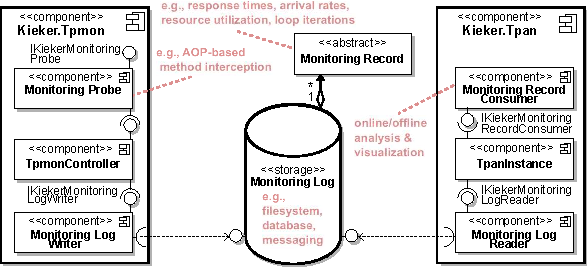
\includegraphics[width=1.0\textwidth]{kiekerComponentDiagram.pdf}
		\label{image:componentdiagram}
		\caption{\Kieker\ component diagram}
	\end{center}
\end{figure}
As can be seen in figure \ref{image:componentdiagram}, the framework consists mainly of two big parts:
\begin{itemize}
\item \textbf{\KiekerMonitoring}\\
This is the part which is responsible for the logging and the recording of the program behavior. The result of this component are the recorded informations which can then be written into different output streams, like for example into files or into a database.
\item \textbf{\KiekerAnalysis}\\
This part is responsible for the evaluation and visualization of the recorded information. It uses the files (or general any collected data which is available as monitoring records) for the analysis and to produce graphs (e.g. Component-Dependency-Graph).
\end{itemize}

\subsection{What ist the purpose of this tutorial?}
In this tutorial, we will take a closer look at both, the \textbf{\KiekerMonitoring}- and the \textbf{\KiekerAnalysis}-part. That means, we will describe on the one hand how \KiekerMonitoring\ can be used to mark parts of the own sourcecode for \Kieker\ and to let them execute under surveilance, so that the recorded information can be saved in files. On the other hand we will use \KiekerAnalysis\ to visualize our recorded data.\\
We will show how to create and execute a simple example before we go deeper into the parts of the framework.

\section{Quickstart}
\subsection{Downloading and installing \Kieker}
For the monitoring and analysis of the source code, it is necessary to download the \Kieker\ binaries from \KiekerDownloadUrl\ first. Once that is done, the content of the zip- respectively the tar.gz-file should be extracted to any directory, for example ``$\sim$/kieker'' (under Linux) or ``c:$\backslash$program files$\backslash$kieker'' (under Windows).\\
That is already enough for the ``installation'' of \Kieker.

\subsection{Monitoring}
Now for the creation of a simple example for the use of the \Kieker\ framework. It is recommended to create a new working directory (e.g. $\sim$/example) with the following subdirectories:
\begin{itemize}
  \item src (For the sourcecode files)
  \item lib (For the libraries and needed jar-files)
  \item META-INF (For the configuration files of \Kieker)
  \item build (For the builded class files of Java)
\end{itemize}
Before we start with the sourcedoe, we need to copy some files from the \Kieker\ directory to our own working directory\footnote{It would be possible to access the required files within the \Kieker\ directory, but the copying will make the compiling much more comfortable.}.
\begin{itemize}
  \item $\sim$/kieker/dist/kieker-tpmon-\version\_ctrl.jar to $\sim$/example/lib/kieker-tpmon-\version\_ctrl.jar
  \item $\sim$/kieker/dist/kieker-common-\version.jar to $\sim$/example/lib/kieker-common-\version.jar
  \item $\sim$/kieker/lib/commons-logging-\version.jar to $\sim$/example/lib/commons-logging-\version.jar
  \item $\sim$/kieker/META-INF/tpmon.properties.example to $\sim$/META-INF/\textbf{tpmon.properties}
  \item $\sim$/kieker/META-INF/log4j.properties.example to $\sim$/META-INF/\textbf{log4j.properties}
\end{itemize}
The last two files are configuration files, but for a quick start they are already configurated correctly.\\

We start with creating two directories for our packages:
\begin{itemize}
  \item $\sim$/example/src/mySimpleKiekerExample
  \item $\sim$/example/src/mySimpleKiekerExample/bookstoreTracing
\end{itemize}
In the last directory, we create three files: 
\begin{itemize}
  \item CRM.java
  \item Catalog.java
  \item Bookstore.java
\end{itemize}
The file ``Bookstore.java'' should contain of the lines showed in listing \ref{listing:Bookstore.java}.

\setJavaCodeListing

\lstset{caption=Bookstore.java, label=listing:Bookstore.java}
\lstinputlisting{source-example/Bookstore.java}
Listing \ref{listing:Catalog.java} shows the content of ``Catalog.java'' and listing \ref{listing:CRM.java} the content of ``CRM.java''.
\lstset{caption=Catalog.java, label=listing:Catalog.java}
\lstinputlisting{source-example/Catalog.java}
\lstset{caption=CRM.java, label=listing:CRM.java}
\lstinputlisting{source-example/CRM.java}

\subsection{Analysis}

\section{\KiekerMonitoring}
\subsection{Configuration}
\subsection{Probes}
\subsection{Writers}

\section{\KiekerAnalysis}
\subsection{Configuration}
\subsection{Readers}
\subsection{Consumers}

\section{Appendix}
\subsection{Example logs}
\subsection{Shortcut via ant}
\subsection{Libraries}
\begin{center}
\begin{longtable}{|p{0.4\textwidth}|p{0.5\textwidth}|}
\hline 
Filename & Description\\
\hline
\hline 
commons-cli-1.2.jar & n/a\\
\hline 
maven & n/a\\
\hline 
mysql-connector-java-5.1.5-bin.jar & The library to connect to an existing MySQL database.\\
\hline 
spring-web.jar & n/a\\
\hline 
Scenario.jar & n/a\\
\hline 
sequence.pic & n/a\\
\hline 
openjms-0.7.7-beta-1.tar.gz & n/a\\
\hline 
aspectjrt-1.6.6.jar & n/a\\
\hline 
commons-logging-1.1.1.jar & n/a\\
\hline 
aspectjtools-1.6.6.jar & n/a\\
\hline 
jms-1.1.jar & n/a\\
\hline 
concurrent-1.3.4.jar & n/a\\
\hline 
servlet.jar & n/a\\
\hline 
pmd & n/a\\
\hline 
spring.jar & n/a\\
\hline 
openjms-common-0.7.7-beta-1.jar & n/a\\
\hline 
servlet-api.jar & n/a\\
\hline 
commons-pool-1.2.jar & n/a\\
\hline 
derby.jar & This library contains the necessary drivers for the Apache Derby database.\\
\hline 
commons-io-1.2.jar & n/a\\
\hline 
cxf-rt-core-2.2.6.jar & n/a\\
\hline 
jmc.jar & n/a\\
\hline 
log4j-1.2.15.jar & n/a\\
\hline 
openjms-net-0.7.7-beta-1.jar & n/a\\
\hline 
aspectjweaver-1.6.6.jar & n/a\\
\hline 
cxf-api-2.2.6.jar & n/a\\
\hline 
rabbitmq-client.jar & n/a\\
\hline 
openjms-0.7.7-beta-1.jar & n/a\\
\hline 
spice-jndikit-1.2.jar & n/a\\
\hline 
cxf-rt-bindings-soap-2.2.6.jar & n/a\\
\hline 
cxf-common-utilities-2.2.6.jar & n/a\\
\hline 
jndi-1.2.1.jar & n/a\\
\hline 
\end{longtable}
\label{tabular:libraries}
\end{center}

\subsection{Troubleshooting}
\end{document}
 
